\documentclass[12pt, a4paper]{article}
\usepackage[utf8]{inputenc}
\usepackage{comment, listings, amssymb, hyperref, natbib, graphicx, amsmath, textcomp, breqn, mathtools, csquotes, cancel, enumitem, amsthm, caption}
\usepackage[english]{babel}
\usepackage[svgnames]{xcolor}
\usepackage{tikz} % load after `xcolor`, since `tikz` internally loads `xcolor`

% NEW (16-04-21, 19p49)
\usepackage[margin = 0.6in]{geometry}
\numberwithin{equation}{section}

\theoremstyle{definition}
\newtheorem{thm}{Theorem}[section] % reset theorem numbering for each chapter

\theoremstyle{definition}
\newtheorem{defn}[thm]{Definition} % definition numbers are dependent on theorem numbers
\newtheorem{exmp}[thm]{Example} % same for example numbers
\newtheorem{lemma}[thm]{Lemma} % same for example numbers
\newtheorem{remark}[thm]{Remark} % same for example numbers
\newcommand{\norm}[2]{\left\vert\left\vert #1 \right\vert\right\vert_{#2}}
\newcommand{\inner}[1]{\left\langle #1 \right\rangle}
\newcommand{\epi}[1]{\text{epi($ #1 $) } }

\lstdefinestyle{mystylepython}{
	language=Python,
	basicstyle=\ttfamily,
	commentstyle=\color{green!40!black},
	keywordstyle=\color{blue},
	numberstyle=\tiny\color{gray},
	numbers=left,
	frame=single,
	breaklines=true,
	showstringspaces=false,
	captionpos=b, 
	tabsize=1,  % Adjust as needed
	columns=fullflexible,
}

\lstdefinestyle{mystylebash}{
	language=bash,
	basicstyle=\ttfamily,
	commentstyle=\color{green!40!black},
	keywordstyle=\color{blue},
	numberstyle=\tiny\color{gray},
	numbers=left,
	frame=single,
	breaklines=true,
	showstringspaces=false,
	captionpos=b, 
	tabsize=1,  % Adjust as needed
	columns=fullflexible,
}

\lstset{
	literate={~}{$\sim$}{1} % otherwise tilde's look really ugly in `lstlisting` envs
}

\title{Infra}
% \subtitle{Questions}
\author{Imahn Shekhzadeh \\ \texttt{\href{mailto:email@example.com}{imahn.shekhzadeh@unige.ch}}\normalsize}
\date{\today}

\begin{document}
	\maketitle 
	\tableofcontents
	
	\section*{\large Note}
	
	The commands in this document might only run through if you use the \textit{.bashrc} file provided in App.~\ref{app:bashrc_file}
	
	\newpage
	
	\section{Baobab/Yggdrasil}
	
	\begin{itemize}
		\item To connect to Baobab from your local machine, just type into a terminal: 
		\begin{lstlisting}[style=mystylebash, label=alg:eval, xleftmargin=\parindent]
			eval $(ssh-agent)
			ssh-add /home/imahn/.ssh/id_ed25519_unige_hpc
			ssh shekhza2@login2.baobab.hpc.unige.ch 
			# ssh shekhza2@login1.yggdrasil.hpc.unige.ch
		\end{lstlisting} 
		
		\item Scp into yggdrasil: 
		\begin{lstlisting}[style=mystylebash, label=alg:scp, xleftmargin=\parindent]
			scp file shekhza2@login1.yggdrasil.hpc.unige.ch:/home/users/s/shekhza2/
			# scp -r folder_name shekhza2@login1.yggdrasil.hpc.unige.ch:/home/users/s/shekhza2/
		\end{lstlisting}
		
		\item To see all the machines that are occupied, just type 
		\begin{lstlisting}[style=mystylebash, label=alg:squeue, caption=Squeue commands, xleftmargin=\parindent]
			squeue
			squeue -p cms-uhh # partition
			squeue -u shekhza2 # user
		\end{lstlisting}
		
		\item To find out about your conda environment, just type (e.g. whether you use Anaconda2 or Anaconda3)
		
		\begin{lstlisting}[style=mystylebash, label=alg:conda_info, xleftmargin=\parindent]
			conda info
		\end{lstlisting}
		
		\item 

		\begin{lstlisting}[style=mystylebash, label=alg:jbn_kernel, xleftmargin=\parindent]
			pip install ipykernel 
			python -m ipykernel install --user --name <environment_name> --display-name "customStuff"
		\end{lstlisting}
	
	\end{itemize}

	\newpage 
	
	\section{Bash}
	
	\begin{itemize}
		\item Downloading file from URL and allowing for redirects, 
		
		\begin{lstlisting}[style=mystylebash, label=alg:curl, xleftmargin=\parindent]
			curl -Lo output.out https://url.com
		\end{lstlisting}
	
		\item For this directory structure, 
		
		\begin{lstlisting}[style=mystylebash, label=alg:exmp__dir_struc, xleftmargin=\parindent]
			infra_upd.tex
			infra_upd.log
			infra_upd.aux
			infra_upd.out
			infra_upd.pdf
		\end{lstlisting} 
		
		rename \textit{all} of them via
		
		\begin{lstlisting}[style=mystylebash, label=alg:linux_mv_files_for, xleftmargin=\parindent]
			for file in infra_upd.*; do mv "$file" "${file/infra_upd/infra}"; done
		\end{lstlisting}
		
		What happens is called a 	\href{https://stackoverflow.com/questions/13210880/replace-one-substring-for-another-string-in-shell-script}{\color{blue}substring replacement}. 
		
		\item Appending line to file,
		
		\begin{lstlisting}[style=mystylebash, label=alg:ubuntu__line_appending, xleftmargin=\parindent]
			echo "this is a line" | tee -a output.out # -a: appending, important
		\end{lstlisting}
		
		\item Checking whether provided string (e.g.~via an argument) is empty or not (typically used within conditional statements): 
		
		\begin{lstlisting}[style=mystylebash, label=alg:bash__empty_string_check, caption=Check (e.g.~in if-clause) whether string is empty or not, xleftmargin=\parindent]
			test_sth() {
				local env_name="$1" # bash starts counting indices from 1
				
				if [ -z "$env_name" ]; then # spacing after `[` and before `]` needed
				echo "The string is empty."
				return 1 # return value of 1 indicates error
				fi
			}
		\end{lstlisting}
	
		\item For retrieving all but the first argument, 
		
		\begin{lstlisting}[style=mystylebash, label=alg:bash__args_shift, xleftmargin=\parindent]
			test_sth(){
				shift
				
				echo "all provided args (except the first): $@"
			}
		\end{lstlisting}
		
		\item And of course there is nothing stopping us from doing this $N\geq 1$-times $\dots$ Pseudocode: 
		
		\begin{lstlisting}[style=mystylebash, label=alg:bash__args_shift_gen, xleftmargin=\parindent]
			test_sth(){
				shift
				...
				shift
				
				echo "all provided args (except the first N): $@"
			}
		\end{lstlisting}
		
		If $N$ arguments are not provided, this is \textbf{not} a problem, the code will still run through.
		
		\item Example for an alias:
		
		\begin{lstlisting}[style=mystylebash, label=alg:bash_aliases, xleftmargin=\parindent]
			# forward output
			ts(){
				test_sth "$@"
			}
		\end{lstlisting}
	
		\item Finding out the size of a file or directory,
		
		\begin{lstlisting}[style=mystylebash, label=alg:dir_size, xleftmargin=\parindent]
			du -hs <path_to_file_or_dir> # du -hs file.ext
			
			# for shorter summary (single quotation strings required)
			du -hs <path_to_file_or_dir> | awk '{print $1}'
		\end{lstlisting}
	
		\item When you want to create a new directory and you want all parent directories to be created as well (assuming they don't already exist), do
		
		\begin{lstlisting}[style=mystylebash, label=alg:bash__dir_creation, xleftmargin=\parindent]
			mkdir -p <dir>
		\end{lstlisting}
		
		The \textit{-p} option is safe, since if the directory is already existent, no error will be outputted
		
		\item Searching for all files with a specific extension, e.g. \textit{.ext}: 
		
		\begin{lstlisting}[style=mystylebash, label=alg:bash_find, xleftmargin=\parindent]
			find . -name "*.ext"
			# find . -name "*.png"
		\end{lstlisting}
		
		Note that this can be nicely combined with \textit{grep}.
		
		\item In Bash, using [[ ]] instead of [ ] is preferred, since [[ ]]  is safer and more capable within Bash scripts. Also, within [ ] (where word splitting and filename expansion do occur), it's good practice to double-quote your variables. But it's safe to omit the double-quotes for e.g.~\$\# within [[ ]].
		
		\item Unzipping a file via the CLI, 
		\begin{lstlisting}[style=mystylebash, label=alg:bash_unzip, xleftmargin=\parindent]
			unzip /path/to/file.zip -d /path/to/destination
		\end{lstlisting}
		
		\item Opening a file and automatically scrolling to the bottom,
		
		\begin{lstlisting}[style=mystylebash, label=alg:less__bottom_scroll, xleftmargin=\parindent]
			less +G /path/to/file.ext
		\end{lstlisting}
	
		\item Comparing the contents of two directories,
		\begin{lstlisting}[style=mystylebash, label=alg:bash_diff__dir, xleftmargin=\parindent]
			diff -r --color directory1 directory2 # `-r` for recursive comparison
			diff -rq --color directory1 directory2 # `-q` suppresses the output of differences and only shows which files differ
		\end{lstlisting}
		
		Ignoring files only existent in one of the directories (which treats absent files as empty),
		\begin{lstlisting}[style=mystylebash, label=alg:, xleftmargin=\parindent]
			diff -rq --color --unidirectional-new-file directory1 directory2 
		\end{lstlisting}
		
	\end{itemize}
	
	\newpage 
	\section{Linux}
	\begin{itemize}
	
		\item Under Ubuntu, listing \textit{all} available kernels, 
	
		\begin{lstlisting}[style=mystylebash, label=alg:ubuntu_kernel, caption=Find kernel versions in Ubuntu, xleftmargin=\parindent]
			dpkg --list | grep linux-image
		\end{lstlisting}

		Finding the currently \textit{active} kernel version,
		\begin{lstlisting}[style=mystylebash, label=alg:ubuntu_kernel__current, caption=Current kerel versions in Ubuntu, xleftmargin=\parindent]
			uname -a
		\end{lstlisting}
	
		The \textit{-a} option stands for \textit{appending}, otherwise \textit{tee} overwrites \textit{output.out} (if existent). 

		\item Better colors in CLI: 
		
		\begin{enumerate}
			\item Use monokai color scheme, i.e.~dark gray background (\#272822) with light peach color for the text (\#F8F8F2)
			\item File paths are still displayed in blue, which is suboptimal, to change the color to the better readable cyan-blue color, click on the three horizontal lines in the CLI, then on \textbf{Preferences}, then choose the currently active color, switch to the \textbf{Colors} tab, then go to \textbf{Palette}, click on the blue color \& instead use the color \#66D9EF
		\end{enumerate}
	
		where \textit{-h} stands for human readability and \textit{-s} for summarizing. 
		
		\item Retrieving the number of available CPU resources,
		
		\begin{lstlisting}[style=mystylebash, label=alg:bash__cpu_res, xleftmargin=\parindent]
			echo "$(nproc)"
		\end{lstlisting}
		
		\item It is possible to use colored outputs in Bash. Check the bash function \textit{str\_diff} in App.~\ref{app:bashrc_file}. (Note that the \textit{-e} option is mandatory to enable interpretation of the backslash escapes).
	
		\item Print day and time from CLI,
		
		\begin{lstlisting}[style=mystylebash, label=alg:cli_date, xleftmargin=\parindent]
			echo "$(date +%d_%m_%y-%H_%M_%S)"
			# echo "$(date +%dp%mp%y-%Hp%Mp%S)"
		\end{lstlisting}
	
		\item Seeing the resource consumption,
		\begin{lstlisting}[style=mystylebash, label=alg:htop, xleftmargin=\parindent]
			htop
		\end{lstlisting}
		
		\item If you did an \textit{sshfs} and the connection hung up, kill the connection via
		\begin{lstlisting}[style=mystylebash, label=alg:fusermount, xleftmargin=\parindent]
			fusermount -zu /path/to/dir
		\end{lstlisting}
		
	\end{itemize}
	
	\subsection{Opening Programs from CLI}
	
	\begin{itemize}
		\item Opening the settings from CLI, 
		
		\begin{lstlisting}[style=mystylebash, label=alg:cli_settings, xleftmargin=\parindent]
			gnome-control-center
		\end{lstlisting}
	
		\item Opening VSCode from CLI: 
		
		\begin{lstlisting}[style=mystylebash, label=alg:ubuntu__vscode_file, xleftmargin=\parindent]
			code path_to_file/file_name.ext
		\end{lstlisting}
		
		If a VSCode editor is already open, use the \textit{-n} flag to open the file in a new editor:
		
		\begin{lstlisting}[style=mystylebash, label=alg:ubuntu__vscode_file_new_editor, xleftmargin=\parindent]
			code -n path_to_file/file_name.ext
		\end{lstlisting}
		
		A folder can also be opened directly:
		\begin{lstlisting}[style=mystylebash, label=alg:ubuntu__vscode_dir, caption=Opening VSCode dir from CLI, xleftmargin=\parindent]
			code path_to_dir
		\end{lstlisting}
		
		\item Opening LibreOffice from CLI:
		
		\begin{lstlisting}[style=mystylebash, label=alg:ubuntu__libre_office, xleftmargin=\parindent]
			libreoffice --writer path_to_dir/filename.odt
		\end{lstlisting}
		
		\item Opening an image via the CLI: 
		
		\begin{lstlisting}[style=mystylebash, label=alg:ubuntu_eog, xleftmargin=\parindent]
			eog /path/to/your/image.jpg
		\end{lstlisting}
	
	\end{itemize}
	
	\newpage 
	
	\section{Anaconda}
	
	\subsection{Installation of Environments}
	
	\begin{itemize}
		\item Installing conda with specific python version,
		
		\begin{lstlisting}[style=mystylebash, label=alg:conda_env__creation_activation, xleftmargin=\parindent]
			# only `myenv` needs to be specified (quotation marks necessary)
			env_name="myenv" && conda create -n "$env_name" python=3.11.3 -y && conda activate "$env_name"
		\end{lstlisting} 
	
		As of Oct 16, I wouldn't recommend installing python 3.12.0 yet (I got a lot of unmet dependency problems when trying to install torch 2.1 with NVIDIA Cuda version 11.8 afterwards). 
		
		\item Installation of conda environment from bash file: 
		
		\begin{lstlisting}[style=mystylepython, label=alg:conda_env__from_bash, xleftmargin=\parindent]
			conda deactivate # go into base environment
			source conda/filename.sh
			touch .env 
		\end{lstlisting}
		
		\item Completely remove conda environment, 
		
		\begin{lstlisting}[style=mystylebash, label=alg:conda_removal, xleftmargin=\parindent]
			conda deactivate && conda remove -n custom-env-name --all -y 
		\end{lstlisting}
	
	\end{itemize} 

	\subsection{Export}
	
	\begin{itemize}
		\item Exporting an yml-file to share with others for reproducibility,
		
		\begin{lstlisting}[style=mystylebash, label=alg:conda_export, xleftmargin=\parindent]
			conda env export > environment.yml
		\end{lstlisting}
		
		At the end of the file, there will be a line starting with \enquote{Prefix:}, you can safely delete it, for details see \href{https://stackoverflow.com/questions/39280638/how-to-share-conda-environments-across-platforms}{here}
	\end{itemize}
	
	\subsection{Installation \& Removal of Packages}
	
	\begin{itemize} 
	
		\item Installation of packages from \textit{pyproject.toml} file, 
		
		\begin{lstlisting}[style=mystylebash, label=alg:pyproject_install, xleftmargin=\parindent]
			pip install -e . 
		\end{lstlisting}
	
		\item Installing specific conda package version:
		
		\begin{lstlisting}[style=mystylebash, label=alg:conda__spec_env_version, xleftmargin=\parindent]
			conda install -c conda-forge custom-pkg-name -y
			# conda install -c conda-forge cloudpathlib=0.15.1 -y
		\end{lstlisting}
	
		\item Removing list of packages from conda environment: 
		
		\begin{lstlisting}[style=mystylebash, label=alg:conda__remove_pkgs, xleftmargin=\parindent]
			conda remove -n custom-env-name pkg1 pkg2 ... pkgN -y
			# conda remove -n google_jax matplotlib -y
		\end{lstlisting}
		
	\end{itemize}

	\subsection{Usage in VSCode}

	\begin{itemize}
		\item Selecting a conda environment in VSCode, do Ctrl + Shift + P and type \textit{Python: select interpreter}. 
		
		\item Stepping into external code with Python debugger:  \url{https://stackoverflow.com/questions/53594900/visual-studio-code-python-debugging-step-into-the-code-of-external-functions}
		
		
		\item Creating a JSON file, here some instructions: \url{https://code.visualstudio.com/docs/python/debugging}
		
		\item Listing all installed environments, 
		
		\begin{lstlisting}[style=mystylebash, label=alg:conda_env_list, xleftmargin=\parindent]
			conda env list
		\end{lstlisting}
		
	\end{itemize}

		\subsection{PyTorch}
	
	\begin{itemize} 		
		\item Checking whether gpu version of PyTorch is installed, from python shell (\textbf{for this, activate the right conda env first!}): 

		\begin{lstlisting}[style=mystylepython, label=alg:find_out_torch_version, xleftmargin=\parindent]
			import os
			
			import torch 
			
			if __name__ == "__main__": 
				os.path.dirname(torch.__file__)
		\end{lstlisting}
	
		Afterwards, do 
		
		\begin{lstlisting}[style=mystylebash, label=alg:find_out_torch_version_ctd, xleftmargin=\parindent]
			ls -larht <path_from_prev_alg> | grep -E "cuda"
		\end{lstlisting}

		\item If you had installed PyTorch via conda instead of pip, then this is easier, where the \textit{-E} means we are searching for extended regular expressions (\textbf{again activate the right conda env first!}):
		
		\begin{lstlisting}[style=mystylebash, label=alg:conda__find_out_torch_version, xleftmargin=\parindent]
			conda list | grep -E "torch|pytorch" 
			# or `conda list | grep -E "torch|pytorch"`
		\end{lstlisting}
	
	\end{itemize} 
	
	\newpage 
	
	\section{CUDA}
	
	\begin{itemize}
		\item When you need to find out the CUDA version installed, install \textit{nvidia-cuda-toolkit}, but do NOT reboot. After its use, immediately remove this package and any package installed alongside with it!
		
		\item In case NVIDIA drivers do not allow for boot into Ubuntu (e.g.~because you did not uninstall the \textit{nvidia-cuda-toolkit} package): 
		\begin{enumerate}
			\item Boot into an older kernel version of Linux (in order to get there, do a "hard" reboot, and then go into "Advanced options for Ubuntu", and choose an older kernel version). 
			\item Once booted into the older kernel version, I removed `nvidia-cuda-toolkit` and rebooted. 
			\item After a few more hard reboots and booting into the older kenel version, at some point, the newer kernel version was picked up and worker again. 
			\item Now to fix the monitors (because dual-monitor setup didn't work), I had to open the program "Additional Drivers" and change the driver from the open-source version to an NVIDIA proprietary one. 
			\item Then I had to install CUDA according to \url{https://docs.nvidia.com/cuda/cuda-installation-guide-linux/index.html} again. 
			\item For PyTorch to recognize the GPU, I had to reboot. 
		\end{enumerate}
		
	\end{itemize}
	
	
		\newpage 
	\section{Docker}
	\subsection{Installation}
	
	\begin{itemize}
		\item Follow  \href{https://www.digitalocean.com/community/tutorials/how-to-install-and-use-docker-on-ubuntu-20-04}{this great tutorial by DigitalOcean}.
		
		\item To use NVIDIA GPUs (both in PyTorch \& Jax), install the \href{https://docs.nvidia.com/datacenter/cloud-native/container-toolkit/latest/install-guide.html#installing-with-apt}{NVIDIA Container Toolkit}
		
		\item Once done with the installation of the NVIDIA Container Toolkit, proceed with the \href{https://docs.nvidia.com/datacenter/cloud-native/container-toolkit/latest/install-guide.html#configuring-docker}{configuration}. During the configuration, it will be necessary to restart the docker daemon, which you can achieve as follows: 
		
		\begin{lstlisting}[style=mystylebash, label=alg:docker_restart, xleftmargin=\parindent]
			sudo systemctl restart docker
		\end{lstlisting}
			
	\end{itemize}
	
	\subsection{Basics}
	
	\begin{itemize} 
		\item Interactive start of containers: 
		
		\begin{lstlisting}[style=mystylebash, label=alg:docker_id, xleftmargin=\parindent]
			d ps -a # find out ID (also docker container name)
			d start -i ID
		\end{lstlisting}
		
		\item Copying files from local system to docker container and vice versa; \textbf{run both commands from local CLI}
		
		\begin{lstlisting}[style=mystylebash, label=alg:docker_cp, xleftmargin=\parindent]
			d cp file_name container_ID:/target_dir # local -> docker
			d cp container_ID:/file_name dir_name # docker -> local
		\end{lstlisting}
	\end{itemize}
	
	\subsection{Dockerfile}
	
	\begin{itemize}
		\item When you find the command for pulling a docker image on \url{https://hub.docker.com}, e.g.~
		
		\begin{lstlisting}[style=mystylebash, label=alg:dockerhub, xleftmargin=\parindent]
			d pull ubuntu:jammy-20231004
		\end{lstlisting}
		
		then in the Dockerfile, just write 
		
		\begin{lstlisting}[style=mystylebash, label=alg:dockerfile_from, xleftmargin=\parindent]
			FROM ubuntu:jammy-20231004
		\end{lstlisting}
		
		When no tag is specified, by default the \textit{latest} one will be taken. However, using the \textit{latest} tag can potentially cause issues with reproducibility and consistency, because you might pull a different version of the image at different times without knowing it if the latest tag gets updated. \textbf{For more predictable builds, it is advised to use a specific version tag.}
		
		\item Note that the structure of the \textit{docker pull} command is
		
		\begin{lstlisting}[style=mystylebash, label=alg:docker_pull, xleftmargin=\parindent]
			d pull [OPTIONS] NAME[:TAG|@DIGEST]
		\end{lstlisting}
		
		In general, the \textit{NAME} is in the format \textit{repository/image}. If \textit{repository} is not specified, Docker assumes the image is located in the default DockerHub library repository. However, many images (like PyTorch) are hosted under a specific user or organization's namespace on DockerHub, rather than the top-level library. That's why the command for the docker pull (for the latest tag) reads 
		
		\begin{lstlisting}[style=mystylebash, label=alg:docker_pull_exmp, xleftmargin=\parindent]
			d pull pytorch/pytorch
		\end{lstlisting}
		
		\item If using a Docker image like \textit{pytorch/pytorch:latest}, conda is already installed. In this case, the default environment is named \textit{base}, which is a common practice in Docker images with conda -- unless otherwise stated. 
		
		\item Copying local scripts into docker container, 
		
		\begin{lstlisting}[style=mystylebash, label=alg:docker_copy, xleftmargin=\parindent]
			COPY relative/path/to/script.py .
		\end{lstlisting}
		
		From the \href{https://docs.docker.com/engine/reference/builder/#copy}{documentation}:
		
		\begin{quote}
			Multiple $\langle$src$\rangle$ resources may be specified but the paths of files and directories will be interpreted as relative to the source of the context of the build. 
		\end{quote}
		
		It is also important to put the \textit{.} at the end, since it represents the destination in the Docker image where the file should be copied. The dot . refers to the current working directory inside the Docker image, which is determined by the WORKDIR command in the Dockerfile. If WORKDIR is not set, it defaults to the root directory (/) of the image.
		
		Also, each time the script \textit{relative/path/to/script.py} changes, the Dockerfile needs to be rebuilt -- \textbf{however, a cached version will be used, which speeds things up}.
		
		\item Copying local dirs into docker container, 
		
		\begin{lstlisting}[style=mystylebash, label=alg:docker__copy_dir, xleftmargin=\parindent]
			COPY relative/path/to/dir/ .
		\end{lstlisting}
		
		\item Running a Dockerfile:
		
		\begin{lstlisting}[style=mystylebash, label=alg:docker_build, xleftmargin=\parindent]
			d build -f file_name -t img_name .
			d build -f file_name -t img_name:tag_name . # tag name optional, but recommended, e.g. 1.0 (no quotes required)
			# d build -f file_name --no-cache -t [...] # forcing to rebuild from scratch, no cached version is used (only do if really required)
		\end{lstlisting} 
		
		where \textit{Image\_name} will be the name of the newly created image, \textit{Tag\_name} the tag name and \textit{file\_name} the name of the docker file. 
		
		\item Via 
		
		\begin{lstlisting}[style=mystylebash, label=alg:docker__expose_port, xleftmargin=\parindent]
			EXPOSE custom-port-number
			# EXPOSE 80
		\end{lstlisting}
	
		it is possible to expose a port. Note that port exposure is related to network access. Note that even though network access might not be needed, there is still no harm in exposing a port (since an exposure of the port does not make the docker container more vulnerable).
		
	\end{itemize} 
	
	\subsection{Docker images}
	
	\begin{itemize}
		
		\item A Dockerfile does not necessarily need to have the name \textit{Dockerfile}. To pass another name when building the img, do 
		
		\begin{lstlisting}[style=mystylebash, label=alg:docker__build_with_custom_img_name, xleftmargin=\parindent]
			d build -f custom_docker_file .
		\end{lstlisting}
		
		The . specifies the context of the build, which is the current directory in this case. \textbf{I would recommend running this command from the same dir in which \textit{custom\_docker\_file} is located}.
		
		\item Check all available Docker images via
		
		\begin{lstlisting}[style=mystylebash, label=alg:docker__check_avail_imgs, xleftmargin=\parindent]
			d images
		\end{lstlisting}
		
		\item Cleaning up dangling docker images (these are the entries with \textit{$\langle$none$\rangle$} in the repository or tag name in the output of the previous algo):
		
		\begin{lstlisting}[style=mystylebash, label=alg:docker_rm__dangling, xleftmargin=\parindent]
			d image prune -f
		\end{lstlisting}
		
		\item Removing a Docker image -- \textbf{only do this when finished with using the image}
		
		\begin{lstlisting}[style=mystylebash, label=alg:docker_remove, xleftmargin=\parindent]
			d image rm Image_name:Tag
			# d container rm <container_id> # in case some containers are using the image
		\end{lstlisting}
		
	\end{itemize}
	
	\subsection{Docker containers}
	
		\subsubsection{Basics}

		\begin{itemize} 
	
			\item Running Docker images -- without being able to utilize NVIDIA GPUs:
			
			\begin{lstlisting}[style=mystylebash, label=alg:docker_run, xleftmargin=\parindent]
				d run -it img_name # if `tag_name` was not provided
				d run -it img_name:tag_name # if `tag_name` was provided during build (recommended)
			\end{lstlisting}
		
			\item Running Docker images \& utilizing GPUs: 
			
			\begin{lstlisting}[style=mystylebash, label=alg:docker_run_gpus, xleftmargin=\parindent]
				d run --gpus all -it img_name 
				d run --gpus all -it img_name:tag_name # recommended
			\end{lstlisting}
		
			\item To mount a local file to the container at runtime, do
			
			\begin{lstlisting}[style=mystylebash, label=alg:docker__run_volume_mounting, xleftmargin=\parindent]
				d run -v /absolute/path/to/script.py:/path/to/workdir/script.py --gpus all -it img_name 
				d run -v /absolute/path/to/script.py:/path/to/workdir/script.py --gpus all -it img_name:tag_name # recommended, provide `img_name` & `tag_name`
			\end{lstlisting}
		
			The mounting expects \textbf{absolute} file paths on the side of the host machine.
			
			\item Note that you can include the bash command \textbf{pwd} to avoid having to manually pass absolute paths for the mounting
			
			\begin{lstlisting}[style=mystylebash, label=alg:docker_run__with_pwd, xleftmargin=\parindent]
				d run -v $(pwd)/script.py:/path/to/workdir/script.py --gpus all -it img_name:tag_name # recommended, provide `img_name` & `tag_name`
			\end{lstlisting}
		
			If you need the container to reflect changes made to the scripts on the host without rebuilding the image every time, you would use the \textit{-v} flag to mount the directory. If the scripts won't change, or you don't need to reflect changes in real-time, you don't need to mount the directory, as the necessary scripts have already been copied into the image during the build process.
			
			\item It is also possible to directly mount directories:
			
			\begin{lstlisting}[style=mystylebash, label=alg:docker_run__mount_dir, xleftmargin=\parindent]
				d run -v $(pwd)/dir_path:/path/to/workdir --gpus all -it img_name:tag_name
			\end{lstlisting}
		
			Note that the specified directory from the host is mounted into the container at the specified mount point. If there are any existing files or directories in the container at the mount point, they become obscured by the mount.
			
			\item In several cases it can be useful to remove the docker container right after execution:~When you$\dots$
			\begin{itemize}
				\item[$\circ$] $\dots$are running many short-lived containers, like during development or testing,
				\item[$\circ$] $\dots$want to avoid manual cleanup of stopped containers later on,
				\item[$\circ$] $\dots$are running containers for one-off tasks that do not need to persist any state after they are finished.
			\end{itemize}
			
			In this case, 
			
			\begin{lstlisting}[style=mystylebash, label=alg:docker_run__mount_dir_rm, xleftmargin=\parindent]
				d run --rm -v $(pwd)/dir_path:/path/to/workdir --gpus all -it img_name:tag_name
			\end{lstlisting}

			\item It is also possible to mount two separate host directories to two separate directories within the container,
			
			\begin{lstlisting}[style=mystylebash, label=alg:docker_run__mount_sev_dir_rm, xleftmargin=\parindent]
				d run --rm -v $(pwd)/dir_path1:/path/to/workdir1 -v $(pwd)/dir_path2:/path/to/workdir2 --gpus all -it img_name:tag_name
			\end{lstlisting}
			
			This will not cause any overwriting as each \textit{-v} flag creates a unique mount point inside the container. 
			
			\item Finding out the python version of the Docker image
			
			\begin{lstlisting}[style=mystylebash, label=alg:docker__python_version, xleftmargin=\parindent]
				d run -it --rm img_name:tag_name python3 --version
			\end{lstlisting}
			
			This command will immediately remove the container after execution.
			
		\end{itemize}

		\subsubsection{Passing Arguments}
		
		It is possible to pass arguments when running a docker container. 
		
		\begin{enumerate}
			\item Assuming you have a bash script \textit{run\_scripts.sh}, in which a Python script, e.g.
			
			\begin{lstlisting}[style=mystylebash, label=alg:docker_run__pass_arguments, xleftmargin=\parindent]
				#!/bin/sh
				isort /app/scripts/*.py
				black /app/scripts/*.py
				
				python3 -B /app/scripts/test_script.py
				python3 -B /app/scripts/test_anil.py
			\end{lstlisting}
			
			Modify this bash script s.t.~any arguments passed to the CLI when running the docker container are picked up,
			
			\begin{lstlisting}[style=mystylebash, label=alg:docker_run__pass_arguments_mod, xleftmargin=\parindent]
				python3 -B /app/scripts/test_anil.py "$@"
				# python3 -B /app/scripts/test_script.py "$@" # alternative
			\end{lstlisting}
		
			\item Rebuild (!) the docker image.
			
			\item Now run the docker container as follows:
			
			\begin{lstlisting}[style=mystylebash, label=alg:docker_run__pass_arguments_container, xleftmargin=\parindent]
				d run --rm -v $(pwd)/dir_path:/path/to/workdir --gpus all -it img_name:tag_name arg1 arg2
				# d run --rm -v $(pwd)/dir_path:/path/to/workdir --gpus all -it img_name:tag_name --n_ways 1 --k_shots 1 # example
			\end{lstlisting}
			
		\end{enumerate}
	
	\subsubsection{Listing \& Stopping}
	
	\begin{itemize} 
		
		\item Listing all running containers, 
		
		\begin{lstlisting}[style=mystylebash, label=alg:docker__check_all_contain, xleftmargin=\parindent]
			d ps
		\end{lstlisting}
		
		Listing only the container ID (of all running containers),
		
		\begin{lstlisting}[style=mystylebash, label=alg:docker__contains_ids, xleftmargin=\parindent]
			d ps -q
		\end{lstlisting}
		
		\item Stopping a running container,
		
		\begin{lstlisting}[style=mystylebash, label=alg:docker__stop_contain, xleftmargin=\parindent]
			d stop container-ID
		\end{lstlisting}
		
		\item Stopping a running container and removing it,
		
		\begin{lstlisting}[style=mystylebash, label=alg:docker__stop_rem_contain, xleftmargin=\parindent]
			d stop container-ID && d rm container-ID
		\end{lstlisting}
		
	\end{itemize} 
	
	\subsection{Pushing to DockerHub \& HPC}
	
	\begin{enumerate}
		\item First login to Docker via 
		
		\begin{lstlisting}[style=mystylebash, label=alg:docker_login, xleftmargin=\parindent]
			d login -u user_name -p password
		\end{lstlisting}
		
		\item Then follow the instructions from  \href{https://www.youtube.com/watch?v=iqqDU2crIEQ&t=1002s}{this tutorial} (from minute 17:05 on)
		
		\item And then follow the \href{https://doc.eresearch.unige.ch/hpc/applications_and_libraries?s[]=docker}{HPC tutorial from UNIGE}
		
	\end{enumerate}
	
	\newpage 
	
	\section{Python}
	
	\subsection{Config File \& JSON Files}
	
	\begin{itemize}
		\item  When using  argparse  in combination with a JSON configuration file, the JSON keys need to match the long option names specified in \textit{parser.add\_argument} method calls. The argparse module itself does not automatically recognize abbreviated forms from a JSON file.
	\end{itemize} 

	\subsection{Jupyter Notebooks}
	\begin{itemize}
		\item Converting jupyter notebooks into PDFs:
		
		\begin{lstlisting}[style=mystylepython, label=alg:notebooks_to_pdf, xleftmargin=\parindent]
			for nb in /path/one/Notebook1.ipynb /path/two/Notebook2.ipynb [...]
			do
				jupyter nbconvert --to pdf "$nb"
			done 
		\end{lstlisting}
	
		If you have several notebooks in the same directory, 
		\begin{lstlisting}[style=mystylepython, label=alg:notebooks_to_pdf__wildcard, xleftmargin=\parindent]
			for nb in *.ipynb
			do
				jupyter nbconvert --to pdf "$nb"
			done 
		\end{lstlisting}
		
	\end{itemize}
	
	\subsection{Map (Built-In Function)}
	
	\begin{itemize}
		\item Function signature:
		
		\begin{lstlisting}[style=mystylepython, label=alg:map__func_signa, xleftmargin=\parindent]
			map(function, iterable, *iterables)
		\end{lstlisting}
		
		Description provided in the \href{https://docs.python.org/3/library/functions.html#map}{documentation}:
		
		\begin{quote}
			Return an iterator that applies function to every item of iterable, yielding the results. If additional iterables arguments are passed, function must take that many arguments and is applied to the items from all iterables in parallel. With multiple iterables, the iterator stops when the shortest iterable is exhausted. For cases where the function inputs are already arranged into argument tuples, see \textit{itertools.starmap()}.
		\end{quote}		
		
		\item Example usage:~Natively multiplying Python lists elementwise,
		
		\begin{lstlisting}[style=mystylepython, label=alg:map__python_lists_elementwise, xleftmargin=\parindent]
			from typing import List
			
			def multiply(x: List, y: List):
			    return x * y
			
			list_one = [i for i in range(1000)]
			list_two = [j for j in range(1000, 2000)]
			result = list(map(multiply, list_one, list_two)) # `map` is a built-in function, do not use `(list_one, list_two)` in this case
		\end{lstlisting}
		
		\item Example usage:~Converting NumPy arrays into PyTorch tensors,
		
		\begin{lstlisting}[style=mystylepython, label=alg:map__numpy_torch_conv, xleftmargin=\parindent]
			a = np.array([1, 2, 3, 4])
			tensor_list = list(map(torch.from_numpy, (a,))) # list containing tensor, use of additional brackets necessary
		\end{lstlisting}
	
		\item Example usage:~Converting NumPy arrays into PyTorch tensors,
		
		\begin{lstlisting}[style=mystylepython, label=alg:map__numpy_torch_tuple_unpacking, xleftmargin=\parindent]
			a = np.array([1, 2, 3, 4]) 
			b = np.array([5, 6, 7, 8]) 
			a, b = map(torch.from_numpy, (a, b)) # tuple unpacking
		\end{lstlisting}
		
	\end{itemize}
	
	\subsection{PyTorch}
	
		\subsubsection{Leaf Tensors}
			
			\begin{itemize}
				\item If \texttt{requires\_grad=False}, then the tensor will be leaf by convention. If \texttt{requires\_grad=True}, then the tensor will be leaf if it was created directly by the user and is \textbf{not} the result of an operation, e.g.~\texttt{.to(device)} when the tensor is on \texttt{cpu} and \texttt{device="cuda:0"}.
				
				\item However, by definition, leaf tensors themselves do not have a \textbf{gradient function} \texttt{.grad\_fn} \mbox{because} they are not the result of a differentiable operation applied to other tensors, i.e.~\texttt{grad\_fn} on such tensors will return \texttt{None}. The gradient function in neural network libraries like PyTorch or TensorFlow is associated with tensors that are outputs of differentiable operations.
				
				\item The \texttt{.grad} attribute on leaf tensors that require gradients, i.e.~those for which \\ \texttt{requires\_grad=True}, stores the gradient computed during backpropagation. (For leaf tensors that have \texttt{requires\_grad=False}, calling the \texttt{.grad} attribute outputs \texttt{None}.) Note that for non-leaf tensors, calling \texttt{.grad} results in a \texttt{UserWarning}, since non-leaf tensors are generally intermediate results in the computation graph, and their gradients are usually not needed once the gradients of the leaf tensors have been obtained. However, there are cases where those gradients are needed, which can be enforced by setting \texttt{retain\_grad=True} on those tensors,
				
				\begin{lstlisting}[style=mystylepython, label=alg:retain_grad, xleftmargin=\parindent]
					x = torch.tensor([1., 2., 3.], requires_grad=True, device=torch.device("cuda:0"))
					
					# fwd pass
					y = x**2
					
					# retain gradients
					y.retain_grad()

					# backward pas
					y.sum().backward()
					
					# access gradients
					y.grad # `torch.tensor([1., 1., 1.], device="cuda:0")`
				\end{lstlisting}
				
				Note that in the example of this code snippet, doing \texttt{y.grad} means that we access the gradient of the scalar loss function \texttt{y.sum()} --- on which we performed \texttt{.backward()}. Correspondingly, doing \texttt{x.grad} implies the gradient of the scalar loss function \texttt{y.sum()} with respect to \texttt{x}.
				
				\item In general, it is \textbf{not} possible to perform \textbf{in-place} operations on leaf tensors for which \\ \texttt{requires\_grad=True}, since
				PyTorch dynamically builds a computational graph during the forward pass, which is used during backpropagation to calculate the gradients. If leaf tensors that have \texttt{requires\_grad=True} are changed in-place, then the values used during the forward pass are changed, which will affect the gradient calculations in the backward pass. However, note that when no gradients are required for the operations, e.g.~when performing parameter updates manually, one can use the context manager \texttt{with torch.no\_grad()}, in which case in-place operations on leaf tensors \textbf{can} be performed, since inside the context manager, \texttt{requires\_grad=False}.
				
			\end{itemize}		
		
		\subsubsection{Autograd \& Backward}
		
			\begin{itemize}
				\item The function \texttt{torch.autograd.grad()} computes the gradient. If the gradient of a scalar (loss function) wrt a (weight) matrix is taken, then the output will also be a matrix, where each element corresponds to the partial derivative of the scalar (loss function) wrt to the (weight) matrix element.
				
				\item \texttt{torch.autograd.grad()} is particularly useful if more direct control over the gradient computation is desired, in particular compared to \texttt{.backward()}.
				
				\item Note that the default behavior of \texttt{.backward()} accumulates gradients in the \texttt{.grad} attribute of tensors,
				
				\begin{lstlisting}[style=mystylepython, label=alg:torch_backward, xleftmargin=\parindent]
					x = torch.tensor([1., 2., 3.], requires_grad=True, device=torch.device("cuda:0"))
					
					# fwd pass
					y = 2 * x
					
					# first backward pass
					y.sum().backward(retain_graph=True)
					print(f"Gradients of `x` after first backward pass: {x.grad}") # `torch.tensor([2., 2., 2.])`
					
					# second backward pass
					y.sum().backward()
					print(f"Gradients of `x` after second backward pass: {x.grad}")  # `torch.tensor([4., 4., 4.])`, notice how gradients have accumulated
				\end{lstlisting}
				
				However, this behavior can be suppressed by simply zeroing the gradients, i.e.~\texttt{x.grad.zero\_()} --- note that \texttt{x.grad} returns a tensor, and \texttt{<tensor>.zero\_()} is a general PyTorch function that sets all elements in-place to $0$.
			\end{itemize}

	\newpage 
	
	\section{AWS S3} 
	
	\subsection{Installation \& Configuration}
	
	\begin{enumerate}
		\item Installation instructions:~ \url{https://docs.aws.amazon.com/cli/latest/userguide/getting-started-install.html#getting-started-install-instructions}
		\item The CLI will display the path under which the \textit{aws} package was installed, but it might be sufficient to simply run 
		
		\begin{lstlisting}[style=mystylebash, label=alg:aws, xleftmargin=\parindent]
			aws
		\end{lstlisting}
		
		Double check by running 
		
		\begin{lstlisting}[style=mystylebash, label=alg:aws_path, xleftmargin=\parindent]
			which aws
		\end{lstlisting}
		
		\item After installation, configuration is necessary. For this run
		
		\begin{lstlisting}[style=mystylebash, label=alg:aws_configure, xleftmargin=\parindent]
			aws configure
		\end{lstlisting}
		
		You can leave these fields empty:
		
		\begin{lstlisting}[style=mystylebash, label=alg:aws_configure__default_reg, xleftmargin=\parindent]
			Default region name [None]:
			Default output format [None]:
		\end{lstlisting}
		
		A configuration file will be saved under 
		
		\begin{lstlisting}[style=mystylebash, label=alg:aws__config_file, xleftmargin=\parindent]
			~/.aws/credentials
		\end{lstlisting}
		
		\item In the case you are a member of UNIGE, you can obtain the AWS access key ID and the secret access key as follows:
		
		\begin{lstlisting}[style=mystylebash, label=alg:aws__access_secret_key, xleftmargin=\parindent]
			echo -n "$user_name" | base64 # the `-n` is important in this context
			echo -n "$passwd" | md5sum
		\end{lstlisting}
		
		where \$user\_name and \$passwd need to be provided
		
		Otherwise, you need login to the AWS Management Console. 
		
		\item \textbf{To test the configuration was successful, do this:}
		
		\begin{lstlisting}[style=mystylebash, label=alg:aws_configure_test, xleftmargin=\parindent]
			aws s3 ls --endpoint-url https://your-custom-s3-endpoint.com
		\end{lstlisting}
		
		where you replace the endpoint-url \url{https://your-custom-s3-endpoint.com} with yours.
		
	\end{enumerate}

	\subsection{AWS Credentials (Profiles)}
	
	\begin{itemize}
		\item It is possible to use several profiles in the file \textit{$\sim$/.aws/credentials}. 
		\item For example:
		
		\begin{lstlisting}[style=mystylebash, label=alg:aws_profiles, xleftmargin=\parindent]
			[default]
			aws_access_key_id = YOUR_DEFAULT_ACCESS_KEY
			aws_secret_access_key = YOUR_DEFAULT_SECRET_KEY
			
			[profile1]                                                                   
			aws_access_key_id = ANOTHER_ACCESS_KEY_ID
			aws_secret_access_key = ANOTHER_SECRET_ACCESS_KEY
			
			[profile2]
			aws_access_key_id = YET_ANOTHER_ACCESS_KEY_ID
			aws_secret_access_key = YET_ANOTHER_SECRET_ACCESS_KEY
		\end{lstlisting}
	
		To use a specific profile when running \textit{aws cli} commands, you can use the \textit{--profile} option in the command:
		
		\begin{lstlisting}[style=mystylebash, label=alg:aws_cli__profile, xleftmargin=\parindent]
			aws s3 --profile profile1 [...]
			# aws s3 --profile default [...]
		\end{lstlisting}
		
	\end{itemize}

	\subsection{Buckets}
	
	One can have several buckets. 
	
	\subsubsection{Creation}

	\begin{itemize}
		
		\item To create a new bucket:
		
		\begin{lstlisting}[style=mystylebash, label=alg:aws__new_bucket, xleftmargin=\parindent]
			aws s3api create-bucket --bucket custom-bucket-name --endpoint-url https://custom-s3-endpoint.com --profile default
		\end{lstlisting}
	
	\end{itemize} 

	\subsubsection{Listings}

	\begin{itemize} 
		
		\item Directly showing the file contents of an s3 bucket,
		
		\begin{lstlisting}[style=mystylebash, label=alg:aws__bucket_ls, xleftmargin=\parindent]
			aws s3 ls s3://custom-bucket-name --recursive --endpoint-url https://custom-s3-endpoint.com --profile default # `--recursive` optional
		\end{lstlisting}
		
	\end{itemize}

	\subsubsection{File Copying}
	
	\begin{itemize}
		\item Local machine $\longrightarrow$ S3:
		
		\begin{lstlisting}[style=mystylebash, label=alg:aws__file_copying_local_s3, xleftmargin=\parindent]
			aws s3 cp path/to/custom_file.ext s3://custom-bucket-name/path/to/custom_file.ext --endpoint-url https://custom-s3-endpoint.com --profile default
		\end{lstlisting}	
		
		\item S3 $\longrightarrow$ local machine:
		
		\begin{lstlisting}[style=mystylebash, label=alg:aws__file_copying_s3_local, xleftmargin=\parindent]
			aws s3 cp s3://custom-bucket-name/path/to/s3_file.ext custom/destination --endpoint-url https://custom-s3-endpoint.com --profile default
		\end{lstlisting}	
	\end{itemize}

	\subsubsection{Directory Copying}
	
	\begin{itemize}
		\item Local machine $\longrightarrow$ S3:
		
		\begin{lstlisting}[style=mystylebash, label=alg:aws__dir_copying, xleftmargin=\parindent]
			aws s3 sync path/to/dir s3://custom-bucket-name/path/to --endpoint-url      
			https://custom-s3-endpoint.com --profile default
		\end{lstlisting}
		
	\end{itemize}

	\subsubsection{Folder/File Deletion}
	
	\begin{itemize}
		\item Deleting a folder (which is essentially a prefix in S3) and its contents in
		an S3 bucket, 
		
		\begin{lstlisting}[style=mystylebash, label=alg:aws__dir_rm, xleftmargin=\parindent]
			aws s3 rm s3://your-bucket-name/path-to-your-folder --recursive --endpoint-url https://custom-s3-endpoint.com --profile default
		\end{lstlisting}
		
		\item Deleting a file, 
		
		\begin{lstlisting}[style=mystylebash, label=alg:aws__file_rm, xleftmargin=\parindent]
			aws s3 rm s3://your-bucket-name/path-to-your-file.out --recursive --endpoint-url https://custom-s3-endpoint.com --profile default
		\end{lstlisting}
		
	\end{itemize}

	\subsection{Cloudpathlib}
	
	\begin{itemize}
		\item When you use the \href{https://cloudpathlib.drivendata.org/stable/}{cloudpathlib} module, and you want to specify a profile, do this:
		
		\begin{lstlisting}[style=mystylepython, label=alg:aws__cloudpathlib_profile, xleftmargin=\parindent]
			from cloudpathlib import S3Path, S3Client
			
			# Create an S3 client with a specific AWS profile
			s3_client = S3Client(
				aws_access_key_id=aws_access_key_id,
				aws_secret_access_key=aws_secret_access_key,
				endpoint_url=endpoint_url,
				profile_name="profile1", # specify profile here
			)
			
			# Make `client` default:
			client.set_as_default_client()
		\end{lstlisting}
		
	\end{itemize}

	\newpage 
	
	\section{Git}
	
	\subsection{Cloning}
	\begin{itemize}
		\item Cloning a repository via \textit{sshfs} and adjusting the folder name, 
		\begin{lstlisting}[style=mystylebash, label=alg:cloning1, xleftmargin=\parindent]
			git clone <ssh_url> <folder_name>
			# git clone <https_path> <folder_name>
		\end{lstlisting}
	
		\item After moving into the <folder_name> via cd, do 
		\begin{lstlisting}[style=mystylebash, label=alg:cloning3, xleftmargin=\parindent]
			git switch <desired_branch>
		\end{lstlisting}
	\end{itemize}

	\subsection{Remote Branch}

	Creating a local branch and then pushing it remotely,
	
	\begin{lstlisting}[style=mystylebash, xleftmargin=\parindent]
		git push origin <local-branch>
		# git push origin code-dev
	\end{lstlisting}
	
	\subsection{Merging}
	
	\begin{itemize}
		\item Assuming the following commit-history is given,
		
		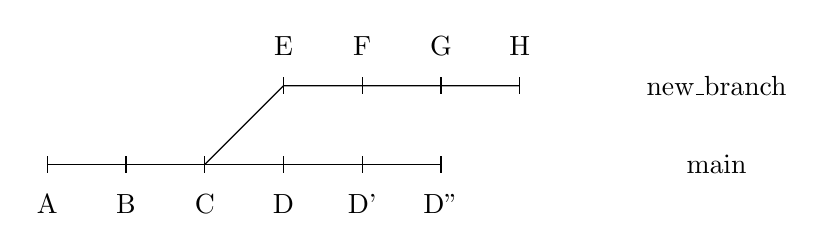
\begin{tikzpicture}
			% Draw the main branch
			\draw (0,0) -- (5,0);
			\foreach \x in {0,1,2,3,4,5}
			\draw (\x cm, 3pt) -- (\x cm, -3pt);
			
			% Label the main branch commits
			\node at (0, -0.5) {A};
			\node at (1, -0.5) {B};
			\node at (2, -0.5) {C};
			\node at (3, -0.5) {D};
			\node at (4, -0.5) {D'};
			\node at (5, -0.5) {D''};
			
			% Draw the new_feature branch
			\draw (2,0) -- (3,1) -- (6,1);
			\foreach \x in {3,4,5,6}
			\draw (\x cm, 1cm + 3pt) -- (\x cm, 1cm - 3pt);
			
			% Label the new_feature branch commits
			\node at (3, 1.5) {E};
			\node at (4, 1.5) {F};
			\node at (5, 1.5) {G};
			\node at (6, 1.5) {H};
			
			% Position the branch labels
			\node[align=left] at (8.5, 0) {main};
			\node[align=left] at (8.5, 1) {new\_branch};
		\end{tikzpicture}
		
		when merging \textit{main} and \textit{new\_branch}, the two branches will be either auto-merged or there will be a merge conflict.
		
		\item Assuming the following commit history is given,
		
		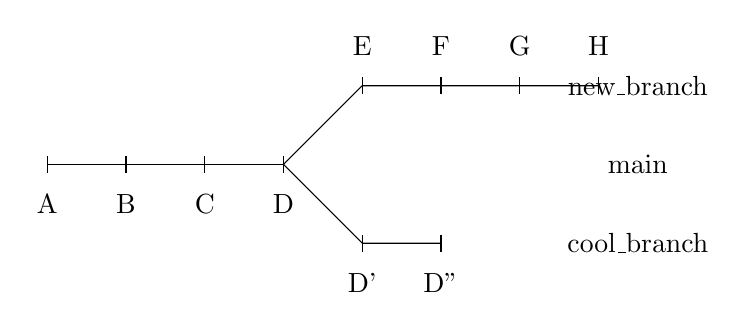
\begin{tikzpicture}
			% Draw the main branch
			\draw (0,0) -- (3,0);
			\foreach \x in {0,1,2,3}
			\draw (\x cm, 3pt) -- (\x cm, -3pt);
			
			% Label the main branch commits
			\node at (0, -0.5) {A};
			\node at (1, -0.5) {B};
			\node at (2, -0.5) {C};
			\node at (3, -0.5) {D};
			
			% Draw the new_feature branch
			\draw (3,0) -- (4,1) -- (7,1);
			\foreach \x in {4,5,6,7}
			\draw (\x cm, 1cm + 3pt) -- (\x cm, 1cm - 3pt);
			
			% Label the new_feature branch commits
			\node at (4, 1.5) {E};
			\node at (5, 1.5) {F};
			\node at (6, 1.5) {G};
			\node at (7, 1.5) {H};
			
			% Draw the cool_feature branch
			\draw (3,0) -- (4,-1) -- (5,-1);
			\foreach \x in {4,5}
			\draw (\x cm, -1cm + 3pt) -- (\x cm, -1cm - 3pt);
			
			% Label the cool_feature branch commits
			\node at (4, -1.5) {D'};
			\node at (5, -1.5) {D''};
			
			% Position the branch labels
			\node[align=left] at (7.5, 1) {new\_branch};
			\node[align=left] at (7.5, -1) {cool\_branch};
			\node[align=left] at (7.5, 0) {main};
		\end{tikzpicture}

		\item After merging \textit{main} with \textit{new\_feature}, which happens via a fast-forward, you can delete it. New commit structure: 
	\end{itemize} 

	\begin{itemize} 
		\item A -- B -- C -- D -- E -- F -- G -- H branch <main>
		\item Merging \textit{new_feature} into \textit{master}, do 
	\end{itemize}

	\begin{lstlisting}[style=mystylebash, label=alg:merging1, xleftmargin=\parindent]
		git switch main
		git merge <new_feature>
	\end{lstlisting}
	
	\subsection{Merge Conflicts}
	
		To resolve a merge conflict, type 
		
		\begin{lstlisting}[style=mystylebash, label=alg:mergetool, xleftmargin=\parindent]
			git mergetool
		\end{lstlisting}

		Afterwards, confirm with Enter that you want to use vimdiff as default editing tool. The vimdiff display will now resemble the following structure: 
		
		\begin{lstlisting}[style=mystylebash, xleftmargin=\parindent]
			| LOCAL | BASE | REMOTE | 
					MERGED
		\end{lstlisting}
		
		If the file has not already existed in BASE, then we need this view: 

		\begin{lstlisting}[style=mystylebash, xleftmargin=\parindent]	
			| LOCAL | MERGED | REMOTE |
			LOCAL  -- Current branch
			BASE   -- Common ancestor (how did the file look like before both changes?)
			REMOTE -- File that I am merging into the current branch
			MERGED -- Merge result
		\end{lstlisting}

		It is probably easiest to take the merged view and edit it directly. In the vim editor, an entire line can be deleted by pressing D (no control before!). 
		If I instead wanted the changes from either LOCAL, BASE or REMOTE, you have to do one of these,
		
		\begin{lstlisting}[style=mystylebash, label=git_merge_view__actions, xleftmargin=\parindent]
			:diffg LO
			:diffg BA
			:diffg LO
		\end{lstlisting}
		
		Of course, the merged view can also be edited directly. Regardless of the chosen method, type 
		
		\begin{lstlisting}[style=mystylebash, xleftmargin=\parindent]
			:wqa
		\end{lstlisting}
		
		into vim. Afterwards, do not forget to commit and push. And if you want, do 
		
		\begin{lstlisting}[style=mystylebash, label=alg:git_clean, xleftmargin=\parindent]
			git clean -f
		\end{lstlisting}

		Locally restore file
		
		\begin{lstlisting}[style=mystylebash, label=alg:git_restore, xleftmargin=\parindent]
			git restore --source <commit SHA> file
			git restore --source HEAD file
		\end{lstlisting}
		
		\textit{git restore} does not overwrite \textit{HEAD}, though. For that, a push would be necessary.  
		
		It can sometimes also be useful to run dry merges to proactively check for conflicts during a merge; for this, run
		
		\begin{lstlisting}[style=mystylebash, label=alg:git__dry_merge, xleftmargin=\parindent]
			git merge --no-commit --no-ff <branch_name>
		\end{lstlisting}

		Afterwards, type 

		\begin{lstlisting}[style=mystylebash, label=alg:git__abort_merge, xleftmargin=\parindent]
			git merge --abort
		\end{lstlisting}
		
		to abort, and no changes will occur.

		If you only want to do a fast-forward, do 

		\begin{lstlisting}[style=mystylebash, label=alg:git__ff_only, xleftmargin=\parindent]
			git merge <branch_to_be_merged> --ff-only
		\end{lstlisting}

	\subsection{Checking History}
	\begin{itemize}
		\item Viewing the history of commits,
		
		\begin{lstlisting}[style=mystylebash, label=alg:history1, xleftmargin=\parindent]
			git log
		\end{lstlisting}
	
		\item Viewing a specific file,
		\begin{lstlisting}[style=mystylebash, label=alg:history1, xleftmargin=\parindent]
			git show <commit-hash>:<file-name>
			# git show 123abc:example.txt
		\end{lstlisting}
	\end{itemize}
	
	\subsection{Removing a File/Folder}
	
	\begin{itemize}
		\item To remove a file/folder that is already tracked, adding it to .gitignore won’t remove it (though this also needs to happen). For this, do:
		
		\begin{lstlisting}[style=mystylebash, label=alg:git_remove, xleftmargin=\parindent]
			git rm --cached <file>
			git rm -r --cached <folder>
		\end{lstlisting}

		\item Adding the file/folder to \textit{.gitignore} is still a good idea, though, since the file/dir won’t be removed locally with the commands.
	\end{itemize}
	
	\subsection{Renaming a Repository}
	
	\begin{enumerate}
		\item Rename the repository remotely first (by going to your repository's URL), 
		\item then go to the locally cloned version of the repository and do
		
		\begin{lstlisting}[style=mystylebash, label=alg:git__rename_repo, xleftmargin=\parindent]
			git remote set-url origin <new-url>
			# git remote set-url origin https://github.com/username/new-repo-name.git 
		\end{lstlisting}
		
		\item and finally 
		
		\begin{lstlisting}[style=mystylebash, label=alg:git__check_remote_url, xleftmargin=\parindent]
			git remote -v
		\end{lstlisting}
		
		which lists the remote names and their URLs.
		
	\end{enumerate}

	\subsection{Restore File}
	
		Resetting specific file to state of previous commit,
		
		\begin{lstlisting}[style=mystylebash, label=alg:git_restore, xleftmargin=\parindent]
			git restore --source=<commit-hash> <file-path>
			# git restore --source=HEAD <file_path>
		\end{lstlisting}
		
		\noindent Replace $\langle$commit-hash$\rangle$ with the commit SHA and $\langle$file-path$\rangle$ with the path to the file. This change is local and you would need to commit it if you want it to be reflected in the repository history.
	
	\subsection{Delete Branches}
	
		\begin{itemize}
			\item Local git branch,
			
			\begin{lstlisting}[style=mystylebash, label=alg:git_delete_branch, xleftmargin=\parindent]
				git branch -d <branch_name>
				# git branch -d testing
			\end{lstlisting}
		
			\item Regardless of merge status,
			
			\begin{lstlisting}[style=mystylebash, label=alg:git_delete_branch__force, xleftmargin=\parindent]
				git branch -D <branch_name>
				# git branch -D testing
			\end{lstlisting}
		
			\item Remote branch,
			
			\begin{lstlisting}[style=mystylebash, label=alg:git_delete_branch__remote, xleftmargin=\parindent]
				git push origin --delete <branch_name>
				# git push origin --delete testing
			\end{lstlisting}
		\end{itemize}
	
	\subsection{List Branches}
		Listing all local and remote branches, 

		\begin{lstlisting}[style=mystylebash, label=alg:git_list_branches, xleftmargin=\parindent]
			git branch -a
		\end{lstlisting}
	
	\subsection{Remote URL}
		Obtaining the remote URL, 
		
		\begin{lstlisting}[style=mystylebash, label=alg:git__remote_url, xleftmargin=\parindent]
			git remote get-url origin 
			git remote get-url origin | sed 's/\.git$//'  # optional: trim output
		\end{lstlisting}
		
	\newpage 
	
	\section{Remote Development}
	
	\subsection{Connection}
	
		\begin{enumerate}
			\item When connecting two machines remotely, install \href{https://marketplace.visualstudio.com/items?itemName=ms-vscode-remote.vscode-remote-extensionpack}{this extension} on local machine (also directly in VSCode possible), 
			\item open VSCode on local machine, 
			\item press F1-button, choose \enquote{Remote-SSH:~Connect to Host...} and type for the SSH host (optionally save it in the SSH config file) the same as in Algo.~\eqref{alg:tailscale_connec}, 
			\item enter the passwd for the remote SSH host. 
		\end{enumerate}	

	\subsection{Troubleshooting}
	
		\begin{itemize}
			\item If you find you are getting a permission error for saving a file on the remote machine (in VSCode when doing the local coding), try
			
			\begin{lstlisting}[style=mystylebash, label=alg:remote_troubleshooting, xleftmargin=\parindent]
				sudo chown custom-username path/to/custom/script.ext
			\end{lstlisting}
			
			The \textit{custom-username} here refers to the username on the remote machine.
			
		\end{itemize}
	
	\newpage	
	
	\section{Jax}
	
	Try to install via pip first. Only if this doesn't work use conda!
	
	\begin{itemize}
		\item To put a Jax array onto a specific device, use this: 
		
		\begin{lstlisting}[style=mystylepython, label=alg:jax_device, caption=Device specification in Jax, xleftmargin=\parindent]
			import jax
			from jax import devices, device_put, numpy as jnp
			
			x = device_put(jnp.arange(10), device=devices("cpu")[0]) # NOTE: put `[0]`
			# x = device_put(jnp.arange(10), device=devices("gpu")[0]) # NOTE: put `[0]`
			print(f"Device: {x.device_buffer.device()}")
		\end{lstlisting}
		
		\item Specifying the dtype of an array: 
		
		\begin{lstlisting}[style=mystylepython, label=alg:jax_dtype, caption=Jax device retrieval, xleftmargin=\parindent]
			x = jnp.array([1, 2, 3], dtype=jnp.float32)
			print(f"Dtype: {x.dtype}")
		\end{lstlisting}
	
		\item To find out the device of a Jax array, use this:
		
		\begin{lstlisting}[style=mystylepython, label=alg:jax__dev_retrieval, caption=Jax device retrieval, xleftmargin=\parindent]
			x.device_buffer.device() # x: Jay array
		\end{lstlisting}
	
		\item To make a Jax array out of a Python list or a \textsc{NumPy} array  (do not use for \textsc{} tensors): 
		
		\begin{lstlisting}[style=mystylepython, label=alg:jax_array_crea, caption=Jax array creation, xleftmargin=\parindent]
			from jax import numpy as jnp
			
			a = jnp.array([1., 2., 3.])
			b = jnp.array(np.array([1., 2., 3.]))
		\end{lstlisting}

		\item jit (just-in-time compilation):~sets up a function with XLA (extended linear algebra):~check out the NB \textit{test\_\_jit-compil.ipynb}. To use jit, do this: 
		
		\begin{lstlisting}[style=mystylepython, label=alg:jax_jit, caption=Jax array, xleftmargin=\parindent]
			import jax
			from jax import numpy as jnp
			
			@jax.jit
			def selu(x: jnp.array, lamb: float = 1., alpha: float = 0.): 
				return lamb * jnp.where(x > 0, x, alpha * (jnp.exp(x) - 1.0))
		\end{lstlisting}
	\end{itemize}

% --------------------------- APPENDIX -------------------------	
	\newpage
	\appendix 
	
	\section{\textit{.bashrc}}
	\label{app:bashrc_file}
	
	\begin{lstlisting}[style=mystylebash, label=alg:bashrc_contents, caption=Contents of .bashrc file, xleftmargin=\parindent]
		ca() {
			local conda_out="$(conda env list | grep -E "$env_name" | head -n 1 | awk '{print $1}')"
			
			# check non-emptiness
			if [ -z "$1" ]; then
				echo "Usage: ca <env_name>"
				return 1
			fi
			
			# check env existence
			if [ ! -z "$conda_out" ]; then
				conda activate "$1"
			else
				echo "Conda environment '$env_name' does not exist." # single quotes (') only for display 
				return 1
			fi
			
		}
		
		# ---------------------------- CONDA ---------------------------
		
		# activate conda environment
		# usage: `ca custom-env-name`
		ca() {
			conda activate "$@"
		}
	
		# deactivate currently activated conda environment
		cod() {
			conda deactivate
		}
		
		# List all available conda envs: 
		cel() {
			conda env list
		}
		
		# remove conda environment
		# usage: `crme ant-migrate-dev` 
		crme() {

			# check number of passed arguments via `$#`
			if [[ $# -ne 1 ]]; then
				echo "NOTE: Exactly one argument needs to be provided"
			else
				conda deactivate && conda remove -n "$1" --all -y
			fi
			
		}
		
		# alias for `conda__remove_packages`
		# usage (e.g.): `crm myenv pkg1 pkg2`
		crm() {
			conda__remove_packages "$@"
		}

		# remove conda packages from environment
		# usage (e.g.): `conda__remove_packages myenv pkg1 pkg2`
		conda__remove_packages() {
			
			# define local variables first
			local env_name="$1"
			local conda_out="$(conda env list | grep -E "$env_name" | head -n 1 | awk '{print $1}')"
			
			# forget first argument (which is saved in `env_name`)
			shift
			
			# check non-emptiness
			if [ -z "$env_name" ]; then
				echo "Usage: conda__remove_packages <env_name> [package1] [package2] ... [packageN]"
				return 1
			fi 
			
			# check env existence
			if [ ! -z "$conda_out" ]; then
				conda remove -n "$env_name" "$@" -y
				echo "Package(s) '$@' removed from environment '$env_name'"
			else
				echo "Conda environment '$env_name' does not exist." # single quotes (') only for display
				return 1	
			fi
			
		}
		
		# ------------------------------- GIT -----------------------------
		
		# list all local and remote branches
		lb() {
			git branch -a
		}

		# delete remote branch
		lbd() {
			git push origin --delete "$@"
		}

		# switch branches and create if non-existent
		lsw() {                                                                                                           
			if git rev-parse --verify "$1" >/dev/null 2>&1; then                                                            
			  git switch "$1"                                                                                               
			else                                                                                                            
			  git switch -c "$1"                                                                                            
			fi                                                                                                              
		}

		# example usage: `lsta 2` or `lsta` 
		lsta() {
			local stash_index=${1:-0}  # Default to 0 if no argument provided
			
			# Check if the provided argument is an integer
			if ! [[ $stash_index =~ ^[0-9]+$ ]]; then
				echo "The provided index is not a valid integer."
				return 1
			fi
			
			# Check if the stash index exists
			if ! git rev-parse --verify stash@{$stash_index} >/dev/null 2>&1; then
				echo "No stash found at index $stash_index"
				return 1  
			fi
			
			# If all checks pass, apply the stash
			git stash apply "stash@{$stash_index}" --index
		}
		
		# Forward commands to `git stash`
		lst() {
			git stash "$@"
		}
		
		# Stash files, if arguments are provided, they are ignored
		lstf() {
			git stash --include-untracked
		}

		# https://stackoverflow.com/questions/19595067/git-add-commit-and-push-commands-in-one
		# https://stackoverflow.com/questions/14763608/use-conditional-in-bash-script-to-check-string-argument
		# if-else statements in bash: https://linuxhandbook.com/if-else-bash/
		# example usage: lgit "bit" "add ..."
		lpush() {
			git add . && git commit -a -m "$1" && git push origin $(bname) && llog
		}
	
		# https://stackoverflow.com/questions/3236871/how-to-return-a-string-value-from-a-bash-function
		bname() {
			branch=$(git branch --show-current)
			echo $branch    
		}
		
		lupd() {
			git fetch origin $(bname) && git log HEAD..origin/$(bname) --oneline
		}
		
		lpull() {
			git pull origin $(bname)
		}
		
		ldiff() {
			git status "$@" && git diff --color "$@"
		}
		
		lforce() {
			git push origin $(bname) --force
		}
		
		llog() {
			git log
		}
		
		lrm() {
			git rm -r "$@"
		}
		
		lreb() {
			# Set default value to 5:
			num1=${1:-5}
			git rebase -i HEAD~$num1
		}
		
		# Reset entire repo to state of `HEAD`, or reset specific file to a specific commit hash.
		lres() {
			if [[ $# -eq 0 ]] || [[ $# -eq 1 ]]; then
				local commit_hash=${1:-HEAD} 
				git reset --hard "$commit_hash"
			elif [ $# -eq 2 ]; then
				local commit_hash="$1"
				local file_path="$2"
				git restore --source="$commit_hash" "$file_path"
			else
				echo "Usage: lres [commit_hash file_path]"
			fi
		} 
		
		lsh(){
			git show "$@"
		}
	
		# Usage: lmv /path/to/directory file1 file2 file3 ... 
		lmv() {
			local target_dir=$1 # The first argument is the directory path                                                
			if [[ ! -d "$target_dir" ]]; then
				echo "Target directory does not exist: $target_dir" >&2
				return 1
			fi
			
			# Shift the arguments so that $@ contains only the files to move                                              
			shift
			
			# Now, loop through all the remaining arguments                                                               
			for file in "$@"; do
				if [[ -e $file ]]; then
					git mv "$file" "$target_dir"
				else
					echo "File does not exist: $file" >&2
				fi
			done
		}
		
		# ---------------------------- PROTONVPN ----------------------

		p() {
			protonvpn-cli "$@"
		}
		
		# ---------------------------- MISCELLANEOUS ------------------
		
		# pdflatex
		pd() {
			/usr/bin/pdflatex "$@"
		}

		# convert input notebook to PDF
		jconv() {
			jupyter nbconvert --to pdf "$1"
		}
		
		# `less` with ANSI escape characters
		less() {
			/usr/bin/less -R "$@"
		}

		diff() {
			/usr/bin/diff --color "$@"
		}

		# overload `shred` func, allow (recursive) shredding of dirs/files
		# multiple files/dirs can be provided, mixing allowed
		# usage (e.g.): `shred 10 <file_name>`
		# shred <file_name>
		# shred <dir_path>
		# shred <file_name> <dir_path>
		shred() {
			
			# check whether first argument is a number
			if [[ "$1" =~ ^[0-9]+$ ]]; then
				local iterations="$1"
				shift
			else
				iterations=5 # default
			fi
			
			# check file/dir existences
			for path in "$@"; do
				if check_existence "$path"; then
				# check whether passed input is directory or not
					if [[ -d "$path" ]]; then
						echo "Files to be shredded in $path:"
						find "$path" -type f -print0 | xargs -0 ls -ld
					fi
				else
					echo "Error occurred in check_existence for file/dir: $path"
					return 1
				fi
			done
			
			# prompt user for confirmation
			read -rp "Do you wish to proceed with shredding all files in $@ for $iterations iterations? (yes/no): " confirmation
			
			if [[ $confirmation = [yY] || $confirmation = [yY][eE][sS] ]]; then
				for path in "$@"; do
					if [[ -d "$path" ]]; then
						# shred all files within the directory
						find "$path" -type f -exec /usr/bin/shred -uz -n "$iterations" {} \;
						rm -rf "$path"
						echo "All files in '$path' have been shredded for $iterations iterations."
					elif [[ -f "$path" ]]; then
						# shred the individual file
						/usr/bin/shred -uz -n "$iterations" "$path"
						echo "File '$path' has been shredded for $iterations iterations."
					fi
				done
			else
				echo "Shredding aborted."
			fi
		}
		
		# shortcut for clearing terminal output
		c() {
			clear
		}
		
		# shortcuts for exiting terminal
		q() {
			exit
		}
		
		e() {
			q
		}
	
		# tailscale 
		ts() {
			tailscale status "$@"
		}
	
		# xournalpp (https://github.com/xournalpp/xournalpp)
		xopp() {
			xournalpp "$@"
		}
	
		# strings comparison
		# usage (e.g.): `str_diff "blub1" "blub1"` or `str_diff blub1 blub1`
		#       or `str_diff $(echo "hey") $(echo "hey")`
		# NOTE: exactly two arguments need to be provided
		str_diff() {
			
			# check number of passed arguments via `$#`
			if [[ $# -ne 2 ]]; then
				echo "NOTE: Exactly two arguments need to be provided"
				return 1 # return non-zero exit code to indicate error
			else
			
				# compare strings
				if [[ $1 == $2 ]]; then
					echo -e "Strings '$1' and '$2' \033[92mmatch\033[0m"
				else
					echo -e "Strings '$1' and '$2' do \033[91mNOT\033[0m match"
				fi
			fi
			
		}
		

		# ----------------------------- DOCKER -----------------------
		d() {
			docker "$@"
		}
	
		# ----------------------------- CHATGPT -----------------------

		# https://github.com/kardolus/chatgpt-cli/tree/main
		gpt(){
			chatgpt -i
		}
	
		export OPENAI_KEY=[...]
	
		# ----------------------------- ALWAYS EXECUTE ----------------
		
		add_bit
		
				
	\end{lstlisting}

\newpage 

\section{Amazing Programs, Extensions, Plugins \& Packages}

	\begin{itemize}
		\item \textbf{\url{https://github.com/charmbracelet/glow}}
		
		\item \textbf{\url{https://github.com/0xacx/chatGPT-shell-cli}}
		
		\item \textbf{\url{https://github.com/kardolus/chatgpt-cli/tree/main}}	
		
		\begin{itemize}
			\item For setting the right model (cf.~\href{https://platform.openai.com/docs/models/gpt-4-and-gpt-4-turbo}{here} for all available models), 
			
			\begin{lstlisting}[style=mystylebash, label=alg:chatgpt_set_model, xleftmargin=\parindent]
				chatgpt --set-model gpt-4-1106-preview --set-max-tokens 128000
			\end{lstlisting}

			\item Usage:

			\begin{lstlisting}[style=mystylebash, label=alg:chatgpt_usage, xleftmargin=\parindent]
				chatgpt -i
			\end{lstlisting}
		\end{itemize}

		\item \textbf{\url{https://tailscale.com/download/}}
		
		\begin{itemize}
			\item Once installation is complete, the command 
			
			\begin{lstlisting}[style=mystylepython, label=alg:tailscale_login, xleftmargin=\parindent]
				sudo tailscale up
			\end{lstlisting}
		
			should be run to login, though this command will also display after installation in the CLI. The signing in should happen via GitHub. To be able to use Tailscale from a new device, it must be added as a device under \url{https://login.tailscale.com/admin/machines}. Once this is done, open a CLI and type 
			
			\begin{lstlisting}[style=mystylepython, label=alg:tailscale_connec, xleftmargin=\parindent]
				ssh name@ip_address # find out <name> and <ip_address> via tailscale console
				# ssh ellie@100.xx.xxx.xx
			\end{lstlisting}
		
			NOTE that if the file already exists locally, it will be overwritten.
			
			\item For file copying (e.g.~from the host machine to the currently used machine), do this
			
			\begin{lstlisting}[style=mystylepython, label=alg:tailscale__scp_file, xleftmargin=\parindent]
				scp name@ip_address:/path/to/remote_file.ext /local/path # find out <name> and <ip_address> via tailscale console
				# ssh ellie@100.xx.xxx.xx
			\end{lstlisting}
			
			For directory copying, 
			
			\begin{lstlisting}[style=mystylepython, label=alg:tailscale__scp_dir, xleftmargin=\parindent]
				scp -r name@ip_address:/path/to/remote_dir /local/path # find out <name> and <ip_address> via tailscale console
				# ssh ellie@100.xx.xxx.xx
			\end{lstlisting}
			
		\end{itemize}
	
		\item \url{https://tailscale.com/kb/1080/cli/} (no separate installation necessary, only tailscale needs to be installed)
		
		\begin{itemize}
			\item Finding out the IPv4 address of the currently active machine,
			
			\begin{lstlisting}[style=mystylepython, label=alg:tailscale_ip, xleftmargin=\parindent]
				tailscale ip -4 
			\end{lstlisting}
			
			\item Finding out the IPv4 address of another machine connected via the Tailscale network,
			
			\begin{lstlisting}[style=mystylepython, label=alg:tailscale_ip, xleftmargin=\parindent]
				tailscale ip -4 custom-name
				# tailscale ip -4 ellie
			\end{lstlisting}
			
		\end{itemize}
		
		\item \url{https://github.com/aws/aws-cli}
		
		\item \url{https://github.com/termcolor/termcolor}
		
	\end{itemize}

\newpage 

\section{VSCode}

	\subsection{Recommended Extensions}
	
		\begin{itemize}
					
			\item  \url{https://marketplace.visualstudio.com/items?itemName=ms-vscode-remote.vscode-remote-extensionpack}
		
			\item \url{https://marketplace.visualstudio.com/items?itemName=Gruntfuggly.todo-tree}
		
		\end{itemize}	

	\subsection{Open the \textit{settings.json} File}\label{app:open_settings_file_vs}
		
		\begin{enumerate}
			\item press Ctrl + Shift + P to the Command Palette, 
			\item type \textbf{Open User Settings (JSON)} and select it to open the \textbf{settings.json} file.
		\end{enumerate}


	\subsection{Fix Unresolved Python Imports}
	
		\begin{itemize}
			\item If you run a docker container where a conda environment is installed (with packages that you do not have locally), then VSCode will show those imports as unresolved. To fix this, open the \textbf{settings.json}, cf.~App.~\ref{app:open_settings_file_vs}, and add the following setting: 
			
			\begin{lstlisting}[style=mystylepython, label=alg:vscode_pylance__unresolved_imports, xleftmargin=\parindent]
				"python.analysis.diagnosticSeverityOverrides": {
				    "reportMissingImports": "none"                          
				}
			\end{lstlisting}
			
			How to incorporate this into the \textbf{settings.json} file is shown in App.~\ref{app:vscode__settings_file}.
			
			\item Note that if you have an SSH connection to another machine going on (e.g.~in the Remote Development extension), then putting the above lines into the \textit{settings.json} file will not have an immediate effect, for this the SSH connection needs to be restarted.
			
		\end{itemize}
	
	\subsection{Opening a Duplicate Workspace}
	
	\begin{enumerate}
		\item press Ctrl + Shift + P to the Command Palette, 
		\item then type \textbf{Workspaces:~Duplicate As Workspace is New Window}
	\end{enumerate}
	
	\subsection{\textit{settings.json}} \label{app:vscode__settings_file}
	
		\begin{lstlisting}[style=mystylebash, label=alg:vscode__settings_file, caption=Contents of settings.json file, xleftmargin=\parindent]
			{
				"workbench.colorTheme": "Default Dark Modern",
				"telemetry.telemetryLevel": "off",
				"editor.wordWrap": "wordWrapColumn",
				"editor.wordWrapColumn": 79,
				"workbench.editor.enablePreview": false,
				"gitlens.telemetry.enabled": false,
				"notebook.lineNumbers": "on",
				"explorer.confirmDragAndDrop": false,
				"window.zoomLevel": 1, 
				"python.analysis.diagnosticSeverityOverrides": {
				    "reportMissingImports": "none"
				 }, 
			 	"todo-tree.general.tags": [
				    "BUG",
				    "HACK",
				    "FIXME",
				    "TODO",
			 	   "NOTE",
				    "XXX",
				    "[ ]",
				    "[x]"
				 ],

				"files.associations": {"*.log": "plaintext"},
				"[plaintext]": {"editor.wordWrap": "off"}, 
				"workbench.editor.tabSizing": "shrink"
			}
		\end{lstlisting}
	
	\newpage 
	
	\section{LibreOffice}
	
	\subsection{Dark Theme}
	
		Go to \textit{Tools} $\rightarrow$ \textit{Options} $\rightarrow$ \textit{LibreOffice} $\rightarrow$ \textit{Application Colors} $\rightarrow$ \textit{Custom Colors} $\rightarrow$ \textit{General} $\rightarrow$ \textit{Document Background} and choose a dark color.

	\newpage 
	
	\section{UNIGE-specific}
	
	\begin{itemize}
		\item Setting up UNIGE e-mail in TB:~\newline\url{https://plone.unige.ch/distic/pub/messagerie/configuration/comment-configurer-compte-office365-thunderbird}
	\end{itemize}
	
\end{document} 